% kernel ridge regression for parameter estimation

%%%%%%%%%%%%%%%%%%%%%%%%%%%%%%%%%%%%%%%%%%%%%%%%%%%
\section{Introduction}
\label{s,krr,intro}
%%%%%%%%%%%%%%%%%%%%%%%%%%%%%%%%%%%%%%%%%%%%%%%%%%%

In MRI \emph{parameter estimation},
one seeks to quantify biomarker ''maps''
(\ie, parameter images) 
from data.
Because MRI acquisitions 
are tunably sensitive
to many physical processes
(\eg, relaxation \cite{bloch:1946:ni-paper}, 
diffusion \cite{torrey:56:bew}, 
and chemical exchange \cite{mcconnell:58:rrb}),
MRI parameter estimation is important
in many QMRI applications
(\eg, relaxometry \cite{bloembergen:1948:rei}, 
diffusivity tensor imaging \cite{bihan:01:dti}, 
and multi-compartmental imaging \cite{mackay:94:ivv}). 
Motivated by such widespread applications,
this chapter describes a method
for fast MRI parameter estimation.

% signal models nonlinear
% so parameter estimation requires nonconvex optimization
% previous chapter described likelihood models
% several works [cite] have had success with this
% however these work for simple problems like single t1/t2 estimation
% for larger problems, undesirable or even intractable
Chapter~\ref{c,relax} applied
a common parameter estimation strategy
to QMRI
that involves minimization
of an objective function
related to the likelihood function
(and possibly regularization terms).
Because MR signal models are typically nonlinear functions
of latent object parameters,
such likelihood-based estimation
requires non-convex optimization in general.
To seek global optima,
several of our 
\cite{nataraj:14:rje,nataraj:14:mbe,nataraj::oms}
and others' 
\cite{staroswiecki:12:seo,ma:13:mrf,beneliezer:15:raa,zhao:16:mlr}
works approach estimation 
via exhaustive grid search,
which requires either storing
or computing on-the-fly a ``dictionary'' 
of scan profile signal vectors.
These works estimate a small (2-3)
number of latent parameters,
and so grid search is practical.
However, 
for even moderately sized problems,
the required number 
of dictionary elements
renders grid search undesirable or even intractable,
unless one assumes artificially restrictive latent parameter constraints.

% clear need for a method that scales well with # parameters?
% multi-compartment: 6-11
% diffusion: at least 7
% phase-based methods: flow, b1, b0, asl? 
There are numerous QMRI applications
that could benefit from an alternative MRI parameter estimation method
that scales well with the number of latent parameters.
For example,
vector (\eg, flow \cite{feinberg:85:mri})
and tensor 
(\eg, diffusivity \cite{bihan:01:dti} or conductivity \cite{tuch:01:ctm})
field mapping techniques
require estimation 
of at minimum 4 and 7 latent parameters per voxel,
respectively.
Phase-based longitudinal \cite{sekihara:85:nif} 
or transverse \cite{morrell:08:aps,sacolick:10:bmb} field mapping
could avoid noise-amplifying algebraic manipulations
on reconstructed image data
that are conventionally used
to reduce signal dependencies 
on nuisance latent parameters.
Compartmental fraction mapping \cite{mackay:94:ivv}
from steady-state pulse sequences
requires estimation of at least 7 \cite{deoni:08:gmt}
and as many as 10 \cite{deoni:13:oct}
latent parameters per voxel.
In these and other applications,
greater estimation accuracy
requires more complete signal models
that involve more latent parameters,
which only increases the need 
for scalable estimation methods.

% omit
% what has been done for larger problems?
% several works tried sim annealing, global opt, region contraction
% however, slow and have been shown to yield constraint-dependent estimates

% kernel methods
% fundamental challenge: nonlinear model
% classical idea: transform nonlinear problem into a linear one
% kernel functions well-suited to make this transformation efficiently
% wahba introduced representation in approx theory
% scholkopf introduced in context of learning theory
% enjoyed success in many machine learning applications,
% originally for classification and later regression
The fundamental challenge 
of scalable MRI parameter estimation
stems from MR signal model nonlinearity:
standard linear estimators
would be scalable but also inaccurate.
One natural solution strategy
involves preprocessing the image data
such that the transformed data 
is at least approximately linear
in the latent parameters.
Without further insight however,
such transformation 
could dramatically increase problem dimensionality,
hindering scalability.
Fortunately, 
a celebrated result
in approximation theory \cite{kimeldorf:70:acb} showed
that simple transformations involving
so-called \emph{reproducing kernel} functions \cite{aronszajn:50:tor}
could accurately represent solutions 
to a relevant class of nonlinear problems
while scaling the associated linear problem's dimensionality 
in a mild, controlled manner.
These kernel methods later found popularity
in machine learning
(initially for classification \cite{cortes:95:svn}
and quickly thereafter for other applications,
\eg regression \cite{saunders:98:rrl})
because they provided simple, scalable nonlinear extensions
to otherwise linear algorithms.

% idea here is to link parameter estimation 
% to a problem of regression
% ideas of machine learning can link estimation (seek parameter estimates from data assuming model) to regression (seek regression function relating 
This chapter introduces a fast, scalable method 
for nonlinear MRI parameter estimation
via kernel ridge regression (KRR).
We observe that 
for voxel-wise separable MRI parameter estimation problems,
one can rapidly simulate many instances
of latent parameter inputs and signal outputs
from the nonlinear signal model.
We take such input-output pairs
as simulated \emph{training points}
and propose to then \emph{learn}
(using an appropriate kernel function)
a nonlinear \emph{regression function}
(\ie, non-iterative estimator)
from the training points.
The proposed KRR-based estimator scales considerably better
with the number of estimated latent parameters
than previously-discussed likelihood-based estimators.

The remainder of this chapter
is organized as follows.
Section~\ref{s,krr,meth}
reviews the general signal model
for an MR scan profile,
constructs an appropriate functional optimization problem,
and efficiently solves this problem using kernels.
Section~\ref{s,krr,pract}
further reduces computational requirements 
via a kernel approximation
and provides guidelines 
for model selection.
Section~\ref{s,krr,exp}
applies KRR-based estimation
to quantify six parameters arising 
from models describing the steady-state 
magnetization dynamics
of two water compartments,
a challenging application
of interest in myelin water fraction imaging 
(discussed in Chapter~\ref{c,mwf}).
Section~\ref{s,krr,summ}
discusses possible extensions 
and provides concluding remarks.

%%%%%%%%%%%%%%%%%%%%%%%%%%%%%%%%%%%%%%%%%%%%%%%%%%%
\section{A Function Optimization Problem \& Kernel Solution}
\label{s,krr,meth}
%%%%%%%%%%%%%%%%%%%%%%%%%%%%%%%%%%%%%%%%%%%%%%%%%%%

Recall from Section~\ref{ss,relax,meth,prof}
that after image reconstruction,
many MRI acquisitions
produce at each voxel position
a sequence of noisy voxel values 
$\bmy \in \complexes{D}$, 
modeled as
\begin{align}
	\bmy = \bms\paren{\bmx; \bmnu} + \bmeps,
	\label{eq:krr,model}
\end{align}
where $\bmx \in \reals{L}$ denotes $L$ \emph{latent} object parameters 
(\eg, relaxation time constants);
$\bmnu \in \reals{K}$ denotes $K$ \emph{known} object parameters 
(\eg, separately acquired and estimated field maps);
$\bms : \reals{L} \times \reals{K} \mapsto \complexes{D}$ 
models the noiseless signals that arise from $D$ datasets;
and $\bmeps \in \complexes{D}$
is complex Gaussian noise,
assumed to be distributed as $\cgauss{\zeros{D}}{\bmSig}$.
Unlike signal models in earlier chapters
(\cf \eqref{eq:scn-dsgn,mod-vec-abbrev}),
Equation~\ref{eq:krr,model} omits
for simplicity
explicit model dependence on acquisition parameters,
as these are fixed 
during parameter estimation.

Here we seek to estimate 
on a per-voxel basis
each latent parameter $\bmx$
from corresponding data sequence $\bmy$ 
and known parameter $\bmnu$.
To develop (or train) a non-iterative estimator $\est{\bmx}$,
we simulate many instances 
of input-output relation \eqref{eq:krr,model}
and use kernels
to develop a nonlinear inverse relation.
We sample $\reals{L} \times \reals{K} \times \complexes{D}$
and evaluate \eqref{eq:krr,model} $N$ times
to produce sets of training inputs
$\set{\paren{\bmx_1,\bmnu_1,\bmeps_1},\dots,\paren{\bmx_N,\bmnu_N,\bmeps_N}}$
and data sequences
$\set{\bmy_1,\dots,\bmy_N}$. 
We seek a function
$\est{\bmh}~:~\reals{Q} \mapsto \reals{L}$
for $Q := 2D+K$
and an offset $\est{\bmb} \in \reals{L}$
that together map each pure-real regressor
$\bmq_n := [\re{\bmy_n}\tpose, \im{\bmy_n}\tpose, \bmnu_n\tpose]\tpose$,
$n \in \set{1,\dots,N}$, 
to an estimate 
$\bmxha{\bmq_n} := \bmhha{\bmq_n}+\est{\bmb}$ 
that is ``close'' to corresponding regressand $\bmx_n$:
\begin{align}
	\paren{\est{\bmh},\est{\bmb}} &\in 
		\set{\argmin{\substack{\bmh \in \hilb^L \\ \bmb \in \reals{L}}}
		\costa{\bmh, \bmb; \paren{\bmx_1,\bmq_1},\dots,\paren{\bmx_N,\bmq_N}}}, 
		\where \label{eq:krr,prob} \\
	\costa{\dots} &= 
		\sum_{l=1}^L \cost_l\paren{h_l,b_l; 
		\paren{x_{l,1},\bmq_1},\dots,\paren{x_{l,N},\bmq_N}}; 
		\label{eq:krr,cost} \\
	\Psi_l(\dots) &= 
		\frac{1}{N} \sum_{n=1}^N \paren{h_l(\bmq_n) + 
		b_l - x_{l,n}}^2 + \rho_l \norm{h_l}_\hilb^2.
	\label{eq:krr,cost-l}
\end{align}
Here, each $h_l~:~\reals{Q} \mapsto \real$ is a scalar function
that maps to the $l$th component of the output of $\bmh$; 
each $b_l,x_{l,n} \in \real$ are scalar components of $\bmb,\bmx$;
$\hilb$ is a (presently unspecified) Hilbert function space,
whose norm $\norm{\cdot}_\hilb$ is
induced by inner product 
$\innprod{\cdot}{\cdot}_\hilb : \hilb \times \hilb \mapsto \real$; 
each $\rho_l$ controls for regularity in $h_l$;
and $\paren{\cdot}\tpose$ denotes vector transpose.

Since \eqref{eq:krr,cost} is separable 
in the components of $\bmh$, 
it suffices to consider optimizing each $\paren{h_l,b_l}$ 
by separately minimizing \eqref{eq:krr,cost-l}
for each $l \in \set{1,\dots,L}$.
Nevertheless, 
minimizing \eqref{eq:krr,cost-l} 
is a challenging functional optimization problem
without further restriction 
on the Hilbert space $\hilb$.
Following many other works involving kernels,
we proceed by hereafter restricting $\hilb$
to be a \emph{reproducing kernel} Hilbert space 
(RKHS) \cite{aronszajn:50:tor}.
Remarkably,
a generalization \cite{scholkopf:01:agr}
of the Representer Theorem \cite{kimeldorf:70:acb},
restated as is relevant here for completeness,
then reduces \eqref{eq:krr,cost-l}
to a finite-dimensional optimization problem:
\begin{thm}[Generalized Representer, \cite{scholkopf:01:agr}]
	Define $k : \reals{Q} \times \reals{Q} \mapsto \real$
	to be the (symmetric positive definite) kernel function 
	associated with RKHS $\hilb$, 
	such that reproducing property $h_l(\bmq) = \innprod{h_l}{k(\cdot,\bmq)}_\hilb$
	holds for all $h_l \in \hilb$ and $\bmq \in \reals{Q}$. 
	Then any minimizer $(\est{h}_l,\est{b}_l)$ of \eqref{eq:krr,cost-l}
	over $\hilb \times \real$
	admits a representation of $\est{h}_l$ of the form
	\label{thm:krr,rep}
	\begin{align}
		\est{h}_l(\cdot) \equiv \sum_{n=1}^N a_{l,n} k(\cdot,\bmq_{n}),
		\label{eq:krr,rep}
	\end{align}
	where each $a_{l,n} \in \real$ for $n \in \set{1,\dots,N}$.
\end{thm}

Theorem~\ref{thm:krr,rep} ensures that any solution to 
\begin{align}
	(\est{\bma}_l,\est{b}_l) \in 
	\set{\argmin{\substack{\bma_l \in \reals{N} \\ b_l \in \real}} 
		\frac{1}{N} \sum_{n=1}^N \paren{\sum_{n'=1}^N a_{l,n'} k(\bmq_n,\bmq_{n'}) 
		+ b_l - x_{l,n}}^2 +
		\rho_l \norm{\sum_{n'=1}^N a_{l,n'} k(\cdot,\bmq_{n'})}^2_\hilb}
	\label{eq:krr,cvx}
\end{align}
corresponds via \eqref{eq:krr,rep} 
to a minimizer of \eqref{eq:krr,cost-l}
over $\hilb \times \real$,
where $\bma_l := [a_{l,1},\dots,a_{l,N}]\tpose$.
Fortunately, a solution of \eqref{eq:krr,cvx} exists uniquely
for $\rho_l > 0$
and can be expressed as
\begin{align}
	\est{\bma}_l &= \inv{\bmM \bmK + N\rho_l\eye{N}} \bmM \bmxg{l};
	\label{eq:krr,a-hat} \\
	\est{b}_l &= \frac{1}{N} \ones{N}\tpose \paren{\bmxg{l} - \bmK \est{\bma}_l},
	\label{eq:krr,b-hat}
\end{align}
where 
$\bmK \in \reals{N \times N}$ is the Gram matrix 
consisting of entries $k(\bmq_n,\bmq_{n'})$ for $n,n' \in \set{1,\dots,N}$;
$\bmM := \eye{N}-\frac{1}{N}\ones{N}\ones{N}\tpose$ is a de-meaning operator;
$\bmxg{l} := [x_{l,1},\dots,x_{l,N}]\tpose$;
$\eye{N} \in \reals{N \times N}$ is the identity matrix;
and $\ones{N} \in \reals{N}$ is a vector of ones.
In the special case where each
$\rho_l \gets \rho$ 
for fixed $\rho>0$, 
corresponding scalar estimators 
$\set{\est{x}_l\paren{\cdot} := \est{h}_l\paren{\cdot} + \est{b}_l}_1^L$
that arise from plugging \eqref{eq:krr,a-hat} into \eqref{eq:krr,rep}
can be concisely concatenated as
\begin{align}
	\bmxha{\cdot} &\gets \bmX 
		\paren{\frac{1}{N}\ones{N} + 
		\bmM\inv{\bmK\bmM + N\rho\eye{N}} \bmka{\cdot}},
		\label{eq:krr,x-hat}
\end{align}
where
$\bmka{\cdot} := 
\brac{k(\cdot,\bmq_1),\dots,k(\cdot,\bmq_N)}\tpose - \frac{1}{N}\bmK\ones{N}
: \reals{Q} \mapsto \reals{N}$
is a kernel embedding operator and 
$\bmX := \brac{\bmx_1,\dots,\bmx_N} = \brac{\bmxg{1},\dots,\bmxg{L}}\tpose 
\in \reals{L \times N}$
collects the regressands. 

% utility of estimate depends on kernel function
% valid kernel is q'*q, which corresponds to linear ridge regression
% more useful kernel is nonlinear fun of q; we use gaussian
For $\rho>0$, 
estimator \eqref{eq:krr,x-hat} minimizes \eqref{eq:krr,cost}
over $\paren{\hilb \times \real}^L$.
However, the utility of \eqref{eq:krr,x-hat}
depends on the choice of kernel $k$,
which induces a choice on the RKHS $\hilb$
and thus the function space $\paren{\hilb \times \real}^L$
over which \eqref{eq:krr,prob} optimizes.
For example, if $k$ was selected as the canonical dot product 
$k(\bmq,\bmq') \gets \innprod{\bmq}{\bmq'}_{\reals{Q}} := \bmq\tpose \bmq'$
(for which RKHS $\hilb \gets \reals{Q}$),
then \eqref{eq:krr,x-hat} would reduce 
to affine ridge regression \cite{hoerl:70:rrb},
which is optimal over $\paren{\reals{Q} \times \real}^L$
but is unlikely to be useful when signal model $\bms$ is nonlinear in $\bmx$.

Since we expect a useful estimate $\est{\bmx}\paren{\bmq}$ 
to depend nonlinearly (but smoothly) on $\bmq$,
we instead use a 
(symmetric, positive definite) 
$k$ that is likewise nonlinear in its arguments
and thus corresponds to a RKHS richer than $\reals{Q}$. 
Specifically, we use a Gaussian kernel
\begin{align}
	k(\bmq,\bmq') \gets \expa{-\frac{1}{2}\norm{\bmq-\bmq'}^2_{\bmL^{-2}}},
	\label{eq:krr,kern}
\end{align}
where symmetric, positive definite 
$\bmL \in \reals{Q \times Q}$ 
controls the length scales in $\bmq$ over which 
the estimator $\est{\bmx}$ smooths.
We focus on the Gaussian kernel
over other candidate kernels
because of its popularity
in the machine learning community 
for representing smooth functions.

Interestingly, 
the RKHS associated 
with Gaussian kernel \eqref{eq:krr,kern}
is infinite-dimensional.
Thus, 
Gaussian KRR
can be interpreted as 
first ``lifting'' 
via a nonlinear \emph{feature map} 
$\bmz : \reals{Q} \mapsto \hilb$ 
each $\bmq$ 
into an infinite-dimensional \emph{feature} $\bmza{\bmq} \in \hilb$,
and then performing affine ridge regression
on the features
via inner products of the form
$k(\bmq,\bmq') \gets \innprod{\bmza{\bmq}}{\bmza{\bmq'}}_{\hilb}$.
From this perspective,
the challenges of nonlinear estimation 
via likelihood models
are avoided 
because we \emph{select} 
(through the choice of kernel) 
characteristics of the nonlinear dependence
that we wish 
for our regression function to model
and need only \emph{estimate} via \eqref{eq:krr,cvx} 
the linear dependence
of $\est{\bmx}$ on the corresponding features.

%%%%%%%%%%%%%%%%%%%%%%%%%%%%%%%%%%%%%%%%%%%%%%%%%%%
\section{Implementation Considerations}
\label{s,krr,pract}

This section focuses
on important practical implementation issues.
Subsection~\ref{ss,krr,pract,apprx} discusses
a scalable and conceptually intuitive approximation
of KRR estimator \eqref{eq:krr,x-hat}.
Subsection~\ref{ss,krr,pract,mod} describes guidelines
for nearly-automatic model selection.

%%%%%%%%%%%%%%%%%%%%%%%%%%%%%%%%%%%%%%%%%%%%%%%%%%%
\subsection{A Kernel Approximation}
\label{ss,krr,pract,apprx}

In practical problems
with even moderately large ambient dimension $Q$,
the necessarily large number of training samples $N$ 
complicates storage of (dense) Gram matrix $\bmK$.
Using a kernel approximation 
can mitigate storage issues.
Here we choose
to sample Random Fourier Features (RFF) \cite{rahimi:07:rff},
a recent method 
for approximating shift-invariants kernels
having form $k\paren{\bmq,\bmq'} \equiv k\paren{\bmq-\bmq'}$.
This subsection reviews the main result of \cite{rahimi:07:rff}
for the purpose of constructing 
an intuitive and computationally efficient approximation of \eqref{eq:krr,x-hat}.

The strategy of \cite{rahimi:07:rff}
is to construct independent probability distributions 
$\dist{\bmv}$ and $\dist{s}$
associated with
random $\bmv \in \reals{Q}$ 
and random $s \in \real$ 
as well as a random function 
(that is parameterized by $\bmq$) 
$\zt\paren{\cdot,\cdot;\bmq} : \reals{Q} \times \real \times \reals{Q} \mapsto \real$,
such that
\begin{align}
	\expect{\bmv,s}{
		\zta{\bmv,s;\bmq}
		\zta{\bmv,s;\bmq'} 
	}
	= k(\bmq-\bmq'),
	\label{eq:krr,exp}
\end{align}
where 
$\expect{\bmv,s}{\cdot}$
denotes expectation with respect to $\dist{\bmv}\dist{s}$.
If such a construction exists,
one can build
approximate feature maps $\bmztZ$
by concatenating evaluations of 
$\ztZ:= \sqrt{2/Z}\zt$ on 
$Z$ samples 
$\set{\paren{\bmv_1,s_1},\dots,\bmv_Z,s_Z}$
of $\paren{\bmv,s}$
(drawn jointly albeit independently),
to produce approximate feature vectors
\begin{align}
	\bmztZa{\bmq} := \brac{\ztZa{\bmv_1,s_1;\bmq},\dots,\ztZa{\bmv_Z,s_Z;\bmq}}\tpose
	\label{eq:krr,feat}
\end{align}
for any $\bmq$. 
Then by the strong law of large numbers,
\begin{align}
	\lim_{Z \to \infty} \innprod{
		\bmztZa{\bmq}}{
		\bmztZa{\bmq'}
	}_{\reals{Z}} \overset{a.s.}{\to} k(\bmq,\bmq') \qquad \forall \bmq,\bmq',
	\label{eq:krr,lln}
\end{align}
which, 
in conjunction 
with strong performance guarantees
for finite $Z$ \cite{rahimi:07:rff,sutherland:15:ote}, 
justifies the interpretation 
of $\bmztZ$ as an approximate 
(and now finite-dimensional) feature map.

We use the Fourier construction 
of \cite{rahimi:07:rff}
that assigns
$\zt\paren{\bmv,s;\bmq} 
\gets 
\cosa{2\pi\paren{\bmv\tpose \bmq + s}}$.
If $s\sim\unif{0,1}$, 
then 
$\expect{\bmv,s}{
		\zt\paren{\bmv,s;\bmq}
		\zt\paren{\bmv,s;\bmq'} 
}$
simplifies to
\begin{align}
	\int_{\reals{Q}} \cosa{2\pi\bmv\tpose\paren{\bmq-\bmq'}} \dist{\bmv}\paren{\bmv} \der{\bmv}.
	\label{eq:krr,ft}
\end{align}
For symmetric positive definite $k$,
\eqref{eq:krr,ft} exists \cite{wu:97:gbt} 
and is the Fourier transform 
% with argument $\paren{\bmq-\bmq'}$
of $\dist{\bmv}$.
Thus, for Gaussian kernel \eqref{eq:krr,kern},
choosing $\bmv\sim\gauss{\zeros{Q}}{\paren{2\pi\bmL}^{-2}}$
satisfies \eqref{eq:krr,exp}.

Subsequent sampling of $\bmv,s$ 
and construction of 
$\bmZt := \brac{\bmztZa{\bmq_1},\dots,\bmztZa{\bmq_N}} \in \reals{Z \times N}$
via \eqref{eq:krr,feat}
gives for $Z \ll N$
a low-rank approximation $\bmZt\tpose\bmZt$ 
of Gram matrix $\bmK$.
Substituting this approximation into \eqref{eq:krr,x-hat}
and applying the matrix inversion lemma \cite{woodbury:50:imm} 
yields
\begin{align}
	\esta{\bmx}{\cdot} \gets \bmmx + \Cxzt\inv{\Cztzt + \rho\eye{Z}} \paren{\bmztZa{\cdot} - \bmmzt},
	\label{eq:krr,x-apx}
\end{align}
where $\bmmx := \frac{1}{N}\bmX\ones{N}$ 
and $\bmmzt := \frac{1}{N}\bmZt\ones{N}$ 
are sample mean vectors; and
$\Cxzt := \frac{1}{N}\bmX\bmM\bmZt\tpose$
and $\Cztzt := \frac{1}{N}\bmZt\bmM\bmZt\tpose$ 
are sample covariance matrices.
Estimator \eqref{eq:krr,x-apx} 
is a regularized variation
of the linear minimum mean-squared error estimator
on the features,
and illustrates
that Gaussian KRR via estimator \eqref{eq:krr,x-hat}
is asymptotically (in $Z$) equivalent
to affine ridge regression
after nonlinear, high-dimensional feature mapping.
%\todo{storage comparison with grid search}

%%%%%%%%%%%%%%%%%%%%%%%%%%%%%%%%%%%%%%%%%%%%%%%%%%%
\subsection{Model Selection}
\label{ss,krr,pract,mod}

This subsection proposes guidelines
for data-driven model selection
through a mixture
of intuitive arguments
and referenced analytical results.
Our goal here is to leave
for uninformed manual tuning
as few model parameters as possible.

\subsubsection{Choosing Sampling Distributions}
\label{sss,krr,pract,mod,dist}

To sample training points,
one must select prior distributions
on object parameters $\bmx,\bmnu$
and noise vector $\bmeps$. 
If offline training is required,
all of these distributions of course
must either be assumed
or empirically estimated
from previous experiments.
Here we focus on online training,
where one trains alongside data processing.

Latent object parameter distributions 
must account for model physics
(to focus samples on useful parameter ranges)
while also leaving generously heavy distribution tails
(to enable precise estimation 
over a broad parameter range).
Known object parameter distributions
can be estimated directly from known $\bmnu$
via density estimation methods, 
\eg \cite{parzen:62:oeo}.
Noise covariance is well-estimated
from low-signal regions of test data.

%\subsubsection{Choosing Number of Training Points $N$}
%\label{sss,krr,pract,mod,n}
% performance bounds (eg, pac statements) likely conservative
% empirical methods: bootstrap?

\subsubsection{Choosing Regularization Parameters}
\label{sss,krr,pract,mod,rho}

% krr from bayesian perspective
% assume x(q) = h(q)+b+eps is a noisy random function with Gaussian process prior
% eps is gaussian noise
% corresponding posterior mean is the krr estimate, with rho <- eps
% here we know selected noise variance, and can estimate cov(x) (when grad full col rank)
Regularization parameter selection is well guided
by considering KRR from an alternative Bayesian formulation.
In this perspective,
the unknown regression function
$\bmh\paren{\cdot}+\bmb$ arises randomly 
from a Gaussian process prior distribution
with mean function zero
and covariance function
given by the kernel.
The observed regressand model
$\bmx\paren{\bmq} = \bmh\paren{\bmq}+\bmb + \bmeps_\bmx$
includes additive \emph{latent parameter noise} $\bmeps_\bmx$ 
because noise is \emph{anticipated} in testing data
and is thus intentionally \emph{simulated} in training data.
If this latent parameter noise is assumed 
to be distributed as 
$\gauss{\zeros{L}}{N\diag{\brac{\rho_1,\dots,\rho_L}\tpose}}$,
then the mean function
of the regression function's posterior distribution
(after observation of training points)
happens to equal the KRR solution 
\eqref{eq:krr,a-hat}-\eqref{eq:krr,b-hat}
for each $l \in \set{1,\dots,L}$
(see \cite[Ch.~2]{rasmussen:05:gpf} for derivations).
In a Bayesian perspective then,
$N\rho_1,\dots,N\rho_L$ should reflect
latent parameter noise covariance.

In MRI parameter estimation,
we can more easily measure noise covariance
in image data $\bmSig$ 
than in latent parameters. 
We relate these two covariances
in the following.

A first-order Taylor expansion
of the signal model 
around $\expect{\bmx}{\bmx}$ is
\begin{align}
	\bmy \approx \expect{\bmy}{\bmy} + 
		\gradxs \paren{\bmx - \expect{\bmx}{\bmx}}.
	\label{eq:krr,model-approx}
\end{align}
Substituting \eqref{eq:krr,model-approx}
into a covariance definition gives
\begin{align}
	\bmSig &= 
		\expect{\bmy}{
			\paren{\bmy - \expect{\bmy}{\bmy}}
			\paren{\bmy - \expect{\bmy}{\bmy}}\ctpose
		}
		\nonumber \\
		&\approx \gradxs \cov{\bmx} \gradxs\ctpose.
		\label{eq:krr,cov-y}
\end{align}
Taking the Moore-Penrose pseudoinverse 
(denoted by $\pinv{\cdot}$)
of each side yields 
\begin{align}
	\gradxs\ctpose \inv{\bmSig} \gradxs &\approx 
		\label{eq:krr,messy} \\
	\gradxs\ctpose \pinv{\gradxs\ctpose} &\inv{\cov{\bmx}} \pinv{\gradxs} \gradxs.
		\nonumber
\end{align}
If the Jacobian matrix $\gradxs$ 
is of full column rank
(and is thus left-invertible), 
Eq.~\eqref{eq:krr,messy} simplifies
after matrix inversion to
\begin{align}
	\cov{\bmx; \bmnu} \approx \inv{\gradxs\ctpose \inv{\bmSig} \gradxs},
	\label{eq:krr,cov-x}
\end{align}
an expression reminiscent
of the \Cramer-Rao Bound 
(\cf Eq.~\eqref{eq:scn-dsgn,fisher}-\eqref{eq:scn-dsgn,crb}).

Expression~\eqref{eq:krr,cov-x} approximates
latent parameter noise covariance 
but is not yet useful
because it remains a function 
of known parameter $\bmnu$,
which varies spatially.
As a simple solution,
one could set regularization parameters $\rho_1,\dots,\rho_L$
using diagonal elements of
\begin{align}
	\inv{N \gradxvs\ctpose \inv{\bmSig} \gradxvs},
	\label{eq:krr,cov-x,approx}
\end{align}
where $\expx$ is taken
with respect to 
the distributions 
used to sample training points 
and $\nubar := \frac{1}{V} \sum_1^V \bmnu\paren{\bmr_v}$
is the sample mean 
of the known object parameters.

Regularization parameter selection 
via \eqref{eq:krr,cov-x,approx}
is extremely fast
but requires signal model gradients
that might be undesirable to compute
or altogether unavailable.
As an alternative,
one could compute the sample covariance matrix
$\Cxx := \frac{1}{N}\bmX \bmM \bmX\tpose$
from simulated training data points 
and set $\rho_1,\dots,\rho_L$
as diagonal elements of $\frac{1}{N}\Cxx$.

\subsubsection{Choosing Smoothing Length Scale}
\label{sss,krr,pract,mod,lam}

With online training,
it is intuitive
to set the Gaussian kernel's 
smoothing length scale 
based on test data sample means
$\bar{\bmy} := \frac{1}{V} \sum_{v=1}^V \bmy\paren{\bmr_v}$
and known parameter sample means $\nubar$:
\begin{align}
	\bmL \gets \lambda_0 
	\diag{\brac{\re{\bar{\bmy}}\tpose, \im{\bar{\bmy}}\tpose, \nubar\tpose}\tpose}.
	\label{eq:krr,length}
\end{align}
Here, $\lambda_0>0$ remains unspecified
as a unitless scalar free parameter
that balances training point consistency 
and estimator regularity.

\subsubsection{Choosing Kernel Approximation Order}
\label{sss,krr,pract,mod,h}

Selection of kernel approximation order $Z$ 
can be guided through performance analysis.  
To this end, 
we apply a bound 
on the expected maximal approximation error 
of RFF \cite{rahimi:07:rff},
studied in Proposition~4 of \cite{sutherland:15:ote}
and restated in our notation below for convenience.
We examine this bound over others
because it requires intuitive selection 
of only one error criterion;
tighter bounds are available,
but may not be as simple to use.
\begin{thm}[\cite{sutherland:15:ote}]
	Let $\setQ$ 
	be a compact subset of $\reals{Q}$
	with diameter $d_\setQ := \sup_{\bmq,\bmq' \in \setQ} \norm{\bmq-\bmq'}_2$.
	Define $k : \setQ \times \setQ \mapsto \real$  
	to be a shift-invariant symmetric positive definite kernel,
	such that $k(\bmq,\bmq') \equiv k(\bmq-\bmq')$
	for each $\bmq,\bmq' \in \setQ$.
	Normalize $k(\zeros{Q}) = 1$ 
	and ensure $\grad^2 k(\zeros{Q})$ exists.
	Further suppose $k$ is $\upsilon$-Lipschitz 
	over $\setQD := \set{\bmq-\bmq'|\bmq,\bmq'\in\setQ}$.
	Construct approximate feature vectors $\bmztZ$
	(defined in \eqref{eq:krr,feat})
	from $Z$ independently drawn samples of $\paren{\bmnu,s}$,
	where $\bmnu$ is distributed 
	with a probability density defined by the Fourier transform of $k$
	and $s \sim \unif{0,1}$.
	Take $r := \expect{\bmnu}{\max\paren{\norm{\bmnu_1}_2,\dots,\norm{\bmnu_Z}_2}}$.
	Assume $\setQ$ and $Z$ are not so small
	as to prevent $\bmztZa{\bmq}\tpose\bmztZa{\bmq'}-k\paren{\bmq,\bmq'}$
	from crossing zero, as is typical. Then
	\label{thm:rff-approx}
	\begin{align}
		\expect{}{\sup_{\bmq,\bmq' \in \setQ} 
			\abs{\bmztZa{\bmq}\tpose\bmztZa{\bmq'}-k\paren{\bmq,\bmq'}}}
			\leq 
			\frac{48 c_\setQ d_\setQ \sqrt{Q}}{\sqrt{Z}} \paren{\upsilon + r},
			\label{eq:krr,rff-approx}
	\end{align}
	where $c_\setQ \in \brac{0.803,1.542}$
	achieves its lower/upper bound for $\setQ$ a ball/sphere.
\end{thm}

For concreteness,
we apply Theorem~\ref{thm:rff-approx} explicitly 
to Gaussian kernel \eqref{eq:krr,kern}.
It suffices to consider $\setQ$ a ball
with diameter 
$d_\setQ \gets 2 
\max\paren{\norm{\bmq\paren{\bmr_1}}_2,\dots,\norm{\bmq\paren{\bmr_V}}_2}$.
Then $c_\setQ \gets 0.803$.
The Gaussian kernel admits a global Lipschitz constant as
\begin{align}
	\upsilon := \sup_{\Delta \in \setQD} \norm{\grada{\Delta}{k}}_2 
		\leq \sup_{\Delta \in \reals{Q}} \norm{\grada{\Delta}{k}}_2 
		= \sqrt{\frac{Q}{e\trace{\bmL^2}}}.
	\label{eq:krr,lipschitz}
\end{align}
The best lower bound we have presently 
for $r$ is 
\begin{align}
	r \leq \frac{1}{2\pi \mineig{\bmL}} \paren{\sqrt{2 \log{Z}} + \sqrt{Q}},
	\label{eq:krr,max-nu}
\end{align}
where $\mineig{\cdot}$ extracts the minimum eigenvalue.
Our overall bound is then 
\begin{align}
	\mathsf{E}&\paren{\sup_{\bmq,\bmq' \in \setQ} 
		\abs{\bmztZa{\bmq}\tpose\bmztZa{\bmq'}-k\paren{\bmq,\bmq'}}} 
		\nonumber \\
	&\leq 
		\frac{96\paren{0.803}
		\paren{\max_v\paren{\norm{\bmq\paren{\bmr_v}}_2}}\sqrt{Q}}{\sqrt{Z}}
		\paren{\sqrt{\frac{Q}{e\trace{\bmL^2}}} + 
		\frac{\sqrt{2 \log{Z}} + \sqrt{Q}}{2\pi \mineig{\bmL}}}
		\label{eq:approx-tight} \\
	&\leq 
		\frac{96\paren{0.803}
		\paren{\max_v\paren{\norm{\bmq\paren{\bmr_v}}_2}}\sqrt{Q}}{\mineig{\bmL}\sqrt{Z}}
		\paren{\frac{1}{\sqrt{e}} + \frac{\sqrt{2\log{Z}} + \sqrt{Q}}{2\pi}}.
		\label{eq:approx-loose}
\end{align}	
Error bound \eqref{eq:approx-tight} is conservative 
due to large constants,
but at least ensures asymptotically
that scaling $Z$ quadratically 
with $Q$ 
will maintain a given expected maximal approximation error tolerance.
Error bound \eqref{eq:approx-loose} is looser,
but more clearly shows 
that selecting $\bmL$ 
via \eqref{eq:krr,length}
makes the bound somewhat invariant
to the scale of test data.

%%%%%%%%%%%%%%%%%%%%%%%%%%%%%%%%%%%%%%%%%%%%%%%%%%%
\section{Experimentation}
\label{s,krr,exp}
%%%%%%%%%%%%%%%%%%%%%%%%%%%%%%%%%%%%%%%%%%%%%%%%%%%

As proof of concept, 
we apply kernel-based estimation 
to quantify parameters describing 
the magnetization dynamics of multiple water compartments,
a challenging application of clinical interest,
\eg, for myelin water imaging 
(application details in Chapter~\ref{c,mwf}).
Specifically,
we use a simple model of two non-exchanging compartments
and seek to estimate the associated latent parameters;
more complex models would only add parameters
and thereby increase the need for an alternative to grid search.

Such challenging estimation problems
typically require multiple data acquisitions
and thus long scans.
To reduce scan times
of classical methods
\cite{mackay:94:ivv},
fast steady-state pulse sequences
were recently proposed 
for two-compartment parameter estimation
\cite{deoni:08:gmt, deoni:11:com}.
We similarly take interest
in steady-state sequences,
but modify acquisition details
to address possible concerns
of insufficient estimation precision
\cite{lankford:13:oti}.

We begin with two-compartment models
of the signals arising from
Spoiled Gradient-Recalled Echo (SPGR)
\cite{zur:91:sot}
and Dual-Echo Steady-State (DESS) 
\cite{bruder:88:ans}
pulse sequences.
We make appropriate assumptions 
to reduce model dependencies
to seven free parameters per voxel:
flip angle spatial variation 
(due to transmit field inhomogeneity) $\stx$;
fast-relaxing compartmental fraction $\ff$;
(spin-lattice, spin-spin) relaxation time constants 
for the fast-relaxing $\paren{\tf{1},\tf{2}}$
and slow-relaxing $\paren{\ts{1},\ts{2}}$ compartments;
and a complex proportionality constant
\footnote{We collect off-resonance effects in $\mzero$
by approximating broadening distributions
to be constant across compartments,
as in prior works \cite{deoni:08:gmt, deoni:11:com}.
We acknowledge this could lead to some bias in practice.}
$\mzero$.
We assume prior knowledge of $\bmnu \gets \stx$ 
(which in practice can be estimated
from separate fast acquisitions, 
\eg \cite{sacolick:10:bmb})
and collect the remaining $L \gets 6$ latent parameters as
$\bmx \gets \brac{\ff,\tf{1},\tf{2},\ts{1},\ts{2},\mzero}\tpose$.

In light of clinical need,
we focus on estimating fast-relaxing fraction $\ff$
and tailor our simulation accordingly.
We optimize 
(by methods similar to those described in Section~\ref{s,scn-dsgn,crb})
the flip angles and repetition times
of four SPGR and three DESS scans
\footnote{Since SPGR (DESS) yields one (two) signal(s) per excitation,
four SPGR and three DESS scans produce a total $D \gets 10$ datasets.}
for precise estimation of $\ff$ 
in white matter (WM) 
and grey matter (GM) regions 
of the human brain.
We consider the other five latent parameters
to be nuisance parameters
and thus do not evaluate the performance of their estimators
in the following.

We simulate data to arise
from two non-exchanging water pools
with nominal fast 
$\paren{\tf{1},\tf{2}} \gets \paren{500,20}$ms
and slow 
$\paren{\ts{1},\ts{2}} \gets \paren{1000,80}$ms
relaxation time constants 
selected from prior measurements 
\cite{mackay:94:ivv,deoni:11:com}.
We assign fast-compartment fractions
$\ff \gets 0.15$ in WM and
$\ff \gets 0.03$ in GM
and constrain corresponding slow-compartment fractions 
as $1-\ff$.
We prescribe these parameter values 
to the anatomy of the BrainWeb digital phantom
\cite{collins:98:dac}
to produce ground truth parameter maps.
Using optimized acquisition parameters
and allowing $\stx$ to model $\pm20\%$ flip angle variation,
we apply two-compartment SPGR and DESS models
to the 81st axial slice of the true parameter maps.
We corrupt these (complex) noiseless signals
with additive complex Gaussian noise
whose covariance $\bmSig \gets \paren{1.49\times10^{-7}} \eye{D\gets10}$
reflects measurements
from normalized datasets \cite{nataraj::oms}.
This yields realistically noisy $217\times181$ (image-domain) datasets
ranging from 24.3-48.8dB SNR in WM
and 26.4-49.5dB SNR in GM.

Because the first and second DESS signals depend differently
on phase accrual due to off-resonance effects \cite{nataraj::oms},
off-resonance related phase (unlike signal loss) 
cannot be collected into $\mzero$.
To avoid (separate or joint) estimation
of an off-resonance field map, 
we elect to estimate parameters 
using magnitude SPGR and DESS image data
and account for consequently Rician-distributed noise
during training.

To sample training points, 
we assume prior distributions 
on latent object parameters $\bmx$
(that distinguish the two compartments
but are otherwise conservative)
and directly measure 
known parameter $\bmnu$ and noise $\bmeps$ distributions
from test data.
We take $\ff$ to be uniformly distributed
on $\brac{-0.1,0.4}$ 
and $\tf{1}$, $\tf{2}$, $\ts{1}$, $\ts{2}$ 
to be log-uniformly distributed
on $\brac{50,700}$ms, $\brac{5,50}$ms, $\brac{700,2000}$ms, $\brac{50,300}$ms,
respectively.
We match the scaling of test data
in training
by taking $\mzero$ 
to be uniformly distributed on $\brac{\eps,u}$, 
where $u$ is set as 5$\times$ the maximum value of test data.
We estimate the distribution of $\bmnu$
via kernel density estimation
\cite{parzen:62:oeo}.
We assume noise covariance $\bmSig$ 
of form $\sigma^2 \eye{10}$
and compute noise variance estimate $\est{\sigma}^2$
from Rayleigh-distributed noise regions
of magnitude test data, using estimators described in 
\cite{siddiqui:64:sif}.

We sample $N \gets 10^6$ training inputs
from these distributions
and use two-compartment SPGR/DESS signal models
to evaluate corresponding (noisy, magnitude) responses.
We set smoothing length scale $\bmL$ 
via \eqref{eq:krr,length},
with $\lambda_0 \gets 1$.
We sample $\paren{\bmv,s}$ $Z \gets 10^3$ times
to construct approximate feature mapping $\bmztZ$.
We apply $\bmztZ$ to training data
and compute sample means $\bmmx$, $\bmmzt$ 
and sample covariance matrices $\Cxzt$, $\Cztzt$, and $\Cxx$.
Lastly, 
we set $\rho_1,\dots,\rho_L$ 
as diagonal entries of $\frac{1}{N}\Cxx$ 
and evaluate \eqref{eq:krr,x-apx}
for each latent parameter
using test datasets and $\stx$ 
on a per-voxel basis. 
On a 3.5GHz desktop computer 
with 32GB RAM
running \matlab R2013a, 
training and estimating 
each took less than 40s and 2s.

\begin{figure*} [!tb]
	\centering
	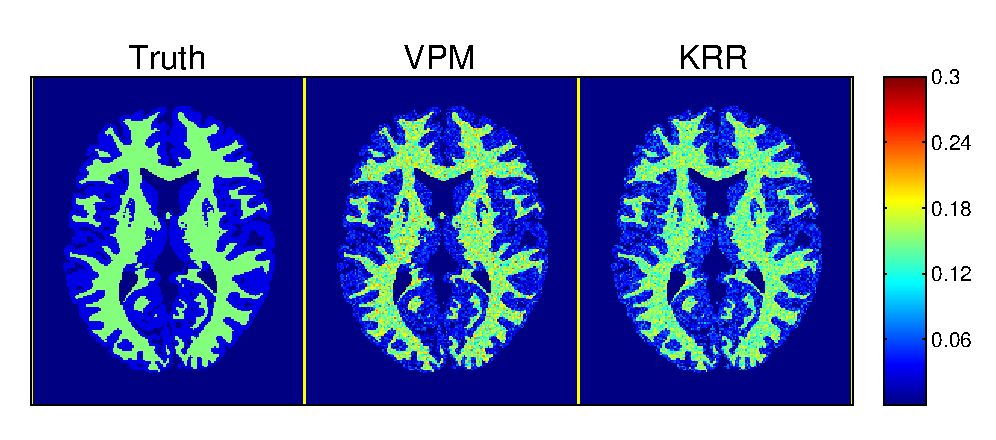
\includegraphics [width=0.81\textwidth] {sim}
	\caption{
		True $\ff$ (\emph{left}) and estimated \ffest
		fast-relaxing compartmental fraction  maps, 
		in simulation.
		Maximum-likelihood estimation 
		via variable projection method and grid search (\emph{center}) 
		is accurate 
		but is computationally expensive.
		In contrast,
		kernel ridge regression (\emph{right}) 
		is very fast and achieves comparable precision,
		at the expense of slightly increased bias
		(\cf Table~\ref{tab:ff}).
		Voxels outside WM/GM regions are masked out 
		in post-processing for visual clarity.
	}
	\label{fig:ff}
\end{figure*}

Fig.~\ref{fig:ff} compares KRR estimates
of fast-relaxing compartmental fraction $\ff$ 
against not only ground truth maps
but also maximum-likelihood estimates
achieved via the ``variable projection'' method (VPM)
\cite{golub:03:snl}
and grid search.
As presented,
the VPM estimate utilizes a dictionary 
of nearly $8 \times 10^6$ signal vectors
computed using finely spaced samples 
on an unrealistically narrow feasible region
consisting of a hypercube 
with boundaries set 
as $\brac{-0.1,0.4}$ in $\ff$
and $\pm20\%$ away from the truth 
in other dimensions.
Using equal computational resources,
estimation via VPM took nearly 4h.

\begin{table}[!t]
	\centering
	\begin{tabular}{c | r | r r}
		\hline
		\hline
		& Truth & VPM & KRR  \\
		\hline
		WM \ffest & $0.15$ 	& \mnstd{0.1538}{0.0292} & \mnstd{0.1440}{0.0221} \\
		GM \ffest & $0.03$ 	& \mnstd{0.0336}{0.0232} & \mnstd{0.0407}{0.0231} \\
		\hline
		\hline
	\end{tabular}
	\caption{
		Sample means $\pm$ sample standard deviations
		of fast-relaxing compartmental fraction estimates \ffest,
		computed over simulated WM- and GM-like voxels.
		Each sample statistic is rounded off
		to the highest place value 
		of its (unreported) standard error,
		which is computed via formulas in \cite{ahn:03:seo}.
	}
	\label{tab:ff}
\end{table}

Table~\ref{tab:ff} reports $\ff$ sample statistics 
computed over $7810$ WM-like and $9162$ GM-like voxels. 
Overall, 
KRR and VPM achieve comparable estimation performance.
In WM,
KRR attains precision slightly higher than
and accuracy similar to VPM.
In GM,
KRR attains precision comparable to
and accuracy slightly lower than VPM.
KRR attains root mean squared errors
lower than VPM in WM ($0.0229$ versus $0.0295$)
and comparable to VPM in GM ($0.0254$ versus $0.0235$).

%%%%%%%%%%%%%%%%%%%%%%%%%%%%%%%%%%%%%%%%%%%%%%%%%%%
\section{Summary and Future Work}
\label{s,krr,summ}
%%%%%%%%%%%%%%%%%%%%%%%%%%%%%%%%%%%%%%%%%%%%%%%%%%%

This chapter has introduced
a fast and computationally efficient method
for MRI parameter estimation
from nonlinear models
via KRR.
As proof of concept,
we applied KRR
to quantify in simulation
fast-relaxing compartmental fraction $\ff$ maps
(along with several nuisance parameters)
using two-compartment signal models
of realistic SPGR and DESS acquisitions.
In \ffest WM/GM regions,
KRR achieved comparable estimation performance
as VPM-accelerated grid search,
with dramatically reduced computation.
Due to its generality,
KRR could potentially accelerate
MRI parameter estimation
in many other applications,
particularly those
involving multiple latent parameters
and/or
cumbersome if not altogether unavailable signal models
(as in, \eg, MR fingerprinting \cite{ma:13:mrf}).



% performance analysis: 
% how must $N$ scale with $L,Q$?
% storage comparison with grid search

% dealing with m0
% adding reconstruction

% -ff range
